\externaldocument{capitulo04}

\chapter{\hspace*{3pt} POR: Processo Objeto - Representação}
\label{chap:por}

A literatura demonstra, que a racionalização do conhecimento é uma área fértil para perspectivas e abordagens distintas. No entanto acreditamos que no âmbito da elaboração de modelos conceituais, uma maneira de representar o conhecimento, perceber os pontos de convergência entre essas teorias pode fornecer um ponto de apoio no processo de representação conceitual acerca de um determinado domínio.

Neste propósito, defendemos que é preciso um processo que seja capaz guiar os modeladores através dos pontos de convergência de maior destaque. Evidenciar a discussão inerente ao processo de construção de modelos conceituais, passando de maneira ativa por cada uma das etapas identificadas e discutidas nas abordagens que servem de fundamentação para este trabalho.

Com base nas teorias apresentadas neste trabalho, elaboramos um fluxo que visa auxiliar a elaboração de modelos conceituais. O processo proposto contempla fases que possuem como propósito guiar o modelador na busca acerca do seus conhecimentos sobre o contexto e como sucedeu sua aquisição. Tal busca, intencional refletir na sua representação mais expressiva e completa.

Este processo, embora esteja dividido em três fases (Percepção, Racionalização e Representação), apresenta sua discussão centrada na fase dois, a racionalização, pois entendemos que esta fase contém o ponto crítico do processo de raciocínio e representação do conhecimento. Em cada fase, identificamos uma ou mais etapas que irão compor o fluxo, que serão apresentadas nas seções seguintes.

A figura \ref{fig:por-resumido} representa essas etapas resumidamente.
\begin{figure}
    \centering
    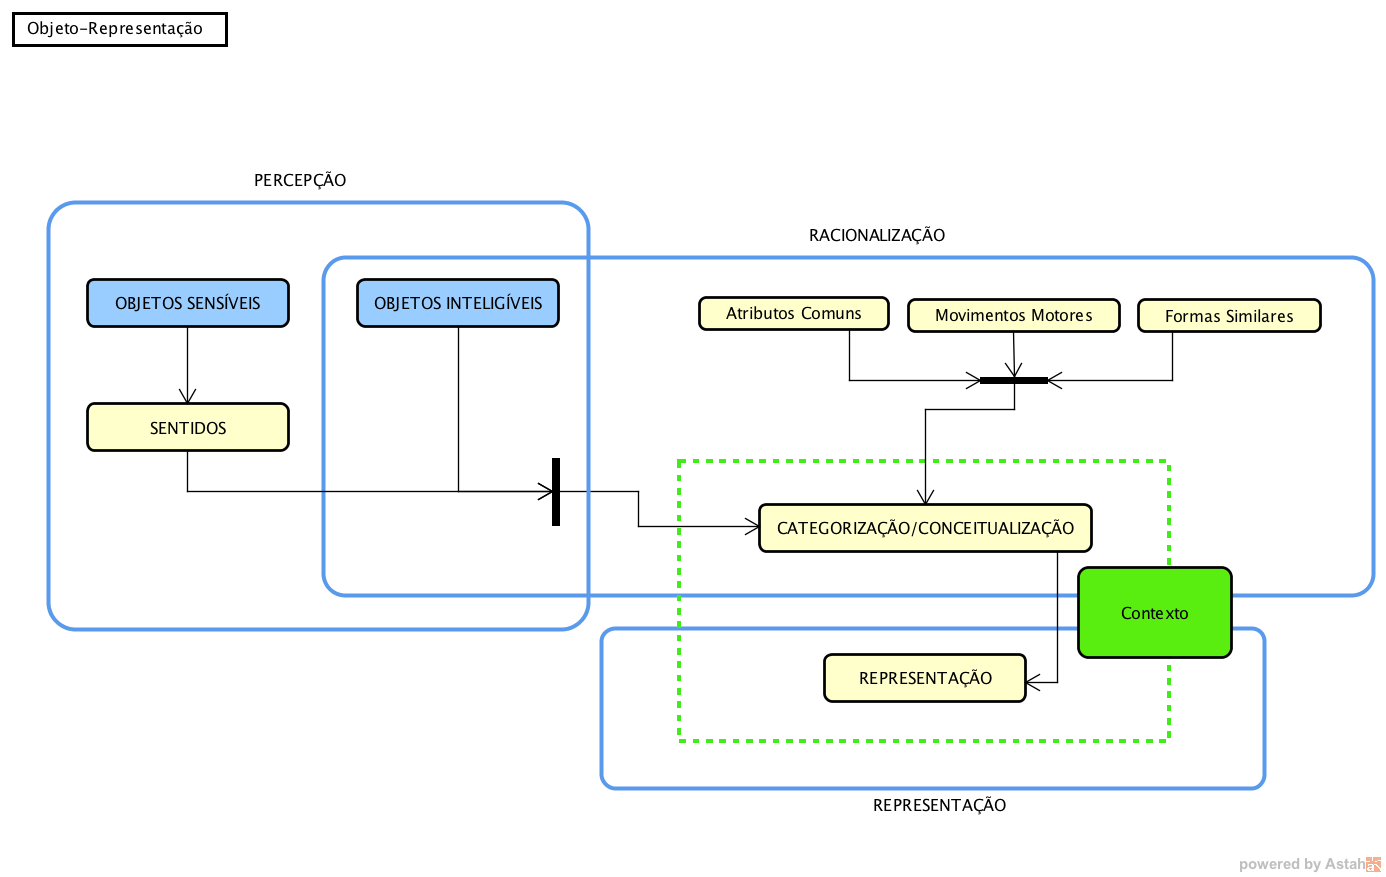
\includegraphics[angle=90, height=\textheight]{imagens/Fases_Processo_O-R.png}
    \caption{Fases do Processo Objeto-Representação}
    \label{fig:por-resumido}
\end{figure}

\section{\hspace*{3pt} Fase 01: Percepção}
\label{sec:percepcao}

A fase um foi definida como a Percepção, cuja função é fornececer os objetos que serão racionalizados. 

Objeto é tudo aquilo que nos circunda ou é designado pelo homem; são as ``coisas" do mundo. Nesta dissertação, o termo ``objeto” é empregado de maneira ampla e pode representar tanto objetos concretos (ex.: um animal ou um veículo), quanto objetos abstratos (ex.: um departamento ou um dragão) \cite{dahlberg:1978.teoria, machado:2009.projeto}. 

Podemos, ainda, categorizá-los em objetos sensíveis, isto é, aqueles objetos que são evidenciados para nós através de um, ou mais, sentidos e objetos inteligíveis, cuja sensação é fruto de um processo mental, como por exemplo a junção de ideias de mulher e peixe, para formar uma sereia ou conceitos que não existem de maneira física, como sentimentos. 

Ao categorizar os objetos em sensíveis e inteligíveis, apesar de reconhecer toda a batalha filosófica travada ao longo dos séculos entre as correntes denominadas Empirismo, Racionalismo e Criticismo, não estamos assumindo uma postura Empirista, mas queremos apenas evidenciar os objetos abstratos, como fruto um processo racional e reflexivo, a despeito de quaisquer discussões filosóficas subjacentes. 

A base da percepção humana são os sentidos, sendo estes estimulados de maneira contínua por um fluxo de acontecimentos. Disto resulta uma excitação neural chamada de sensação \cite{alexandre:2007.factores}.

Sensação, segundo o dicionário online \citeonline{priberam:2015} é ``a impressão produzida pelos objetos exteriores num órgão dos sentidos, transmitida ao cérebro pelos nervos, onde se converte em ideia, julgamento ou percepção''.

Na introdução da Crítica da Razão Pura, \citeonline{kant:1983.critica} afirma que: 

\begin{quote}
``Não há dúvida de que todo o nosso conhecimento começa com a experiência; do contrário, por meio do que a faculdade de conhecimento deveria ser despertada para o exercício senão através de objetos que toquem nossos sentidos e em parte produzem por si próprios representações, em parte põem em movimento a atividade do nosso entendimento para compará-las, conectá-las ou separá-las e, desse modo, assimilar a matéria bruta das impressões sensíveis a um conhecimento dos objetos que se chama experiência? […]" \cite[p.23]{kant:1983.critica}.
\end{quote}
 
Estas impressões, no entanto, são percepcionadas no espaço e no tempo, uma vez que formas puras (vazias) fazem parte das estruturas cognitivas inatas do sujeito. Elas são a condição indispensável para que possamos ter acesso ao conhecimento, isto é, a sensibilidade se expressa em duas formas: espaço e tempo, os  quais, nas palavras de \citeonline{kant:1983.critica}, são definidos, respectivamente, como:

\begin{quote}
``O espaço não é um conceito empírico abstraído de experiências externas. Pois a representação de espaço já tem que estar subjacente para certas sensações se referirem a algo fora de mim […] O espaço é uma representação a priori necessária que subjaz a todas as intuições externas. […] O espaço não é um conceito discursivo ou, como se diz, um conceito universal de relações das coisas em geral, mas sim uma intuição pura. […] O espaço é representado como uma magnitude infinita dada. […] A representação originária do espaço é, portanto, intuição a priori e não conceito" \cite[p.41]{kant:1983.critica}.
\end{quote}

\begin{quote}
``O tempo não é um conceito empírico abstraído de qualquer experiência. […] O tempo é uma representação necessária subjacente a todas intuições. […] Sobre essa necessidade a priori também se funda a possibilidade de princípios apodíticos das relações do tempo, ou de axiomas do tempo em geral. […] O tempo não é um conceito discursivo ou, como se diz, um conceito universal, mas uma forma pura da intuição sensível. […] A infinitude do tempo nada mais significa que toda magnitude determinada do tempo só é possível mediante limitações de um tempo uno subjacente" \cite[p.44--45]{kant:1983.critica}. 
\end{quote}

O espaço e o tempo não são conceitos, visto que não são elaborados pelo sujeito tendo como ponto de partida suas experiências; eles simplesmente existem no sujeito cognoscente, que ao conhecer os objetos do mundo, o fazem de um modo dimensionado e associado à ideia de movimento, de mudança, de evolução, ou mesmo em estágios ou locais diferentes. Por isso as noções de espaço e de tempo são condições necessárias para o conhecimento dos objetos do mundo.

É através de sua percepção que um indivíduo organiza e interpreta suas impressões sensoriais para atribuir significado ao seu meio. Do ponto de vista cognitivo, a percepção envolve processos mentais que interpretam os dados oriundos dos sentidos e os associam aos conceitos.

\section{\hspace*{3pt} Fase 02: Racionalização}
\label{sec:racionalizacao}

A racionalização quem nos permite dar significados aos estímulos que recebemos, transformando os dados oriundos das percepções em ideias ou conceitos.

Esta fase compartilha a visão atomística, que defende que a compreensão de um objeto implica o reconhecimento das partes para ter o entendimento do todo. Embora a visão holística - aquela que defende que a interpretação de um objeto se dá pelo todo - seja reconhecida, o todo quando inserido em um contexto, pode apresentar características que não sejam relevantes para a conceitualização do objeto.

Os experimentos propostos por \citeonline{rosch:1999.principles}, para encontrar o nível médio de abstração: atributos comuns, movimentos motores, forma objetiva e semelhança da forma, ou as forma de conhecer o mundo, quando dentro do contexto, permitem que identifiquemos quais características que são importantes para definição do objeto. 

O contexto delimita no universo do nosso discurso, qual as características dos objetos que percebemos fazem sentidos, e precisam ser compartilhadas para que nossas representações façam sentido para nossos interlocutores.  

A categorização reflete a nossa capacidade para agrupar entidades únicas em conjuntos, usando como regras de agrupamento as características que compartilham entre si. 

\subsection{\hspace*{3pt} Formas de Conhecer o Mundo}

Atributos comuns são as características que dois ou mais objetos de uma mesma categoria compartilham. Ex.: ter bicos, ter penas, por ovos.

Movimentos motores representam a maneira como interagimos determinados objetos, os movimentos musculares associados à utilização do objeto. Ex.: o ato de sentar em uma cadeira ou de cortar com um serrote.

Formas Objetivas e Similares dizem respeito a forma como o objeto se apresenta, isto é, a forma que ele possui. Ex.: cadeira de jantar, cadeira de praia, poltrona.

Nossa experiência associa características novas àquelas percebidas previamente, que sejam semelhantes. Refletir acerca da maneira como as características nos chegam nos ajudam entender como estamos categorizando um determinado grupo de características
            y
